\documentclass[../../main.tex]{subfiles}

\begin{document}

\subsubsection{Sagsåbning}
Sagsbehandlingen i systemet foregår i pakken \code{elucidation}. Det er her al logikken i forhold til udredningen er implementeret. Som det blev beskrevet i afsnit \ref{sec:analyse}, er der blevet analyseret frem til, at \code{CaseWorker} skal have ansvaret for at oprette en sag. I det en bruger er logget ind, bliver en \code{CaseWorker} bundet til \code{Elucidation}. Så når der skal oprettes en sag, går kaldet fra GUI igennem \code{DomainFacade} til \code{elucidation} som kalder \code{createCase()} på den bundne \code{CaseWorker}.

Systemet er implementeret ved at dele GUI-controllere ud i flere klasser, på figur \ref{fig:gui_design}. Bemærk gui pakkens opbygning. Som det ses består \code{GUI} af et antal \code{Controllere}, som for eksempel \code{LoginController}. GUI’en til at oprette en sag består af række controllere, som alle har fællestræk med hinanden, men ikke med den generelle \code{Controller}. Derfor er der implementeret en \code{TabController}, der arver fra \code{Controller}. Denne \code{TabController} arver controllerne der benyttes til at oprette en sag fra.

\begin{center}
\begin{figure}[H]
  \centering
  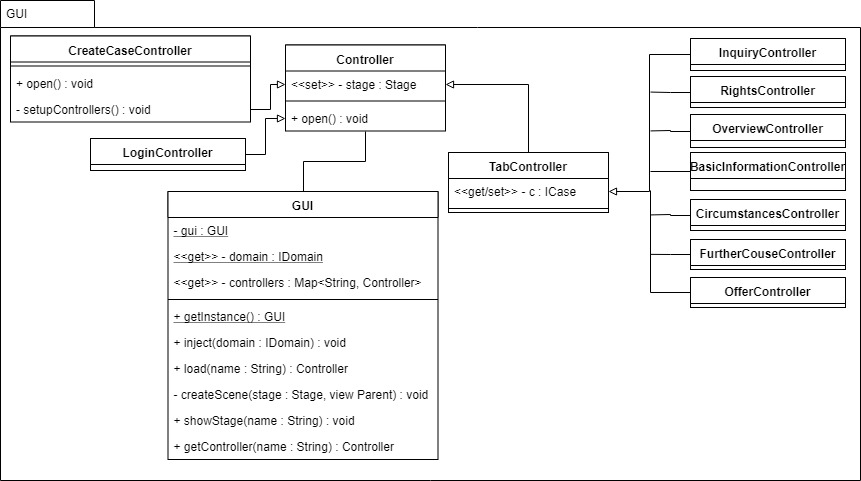
\includegraphics[scale=.5]{figurer/gui_create_case.jpg}
  \caption{Design for GUI'en i systemet}
  \label{fig:gui_design}
\end{figure}
\end{center}

\end{document}
